\documentclass[dvipsnames, svgnames, x11names,border=3pt]{standalone}
\usepackage{tikz,pgfplots}
\usepgfplotslibrary{fillbetween}
\pgfplotsset{compat = 1.18,width=10cm, height=10cm}

\begin{document}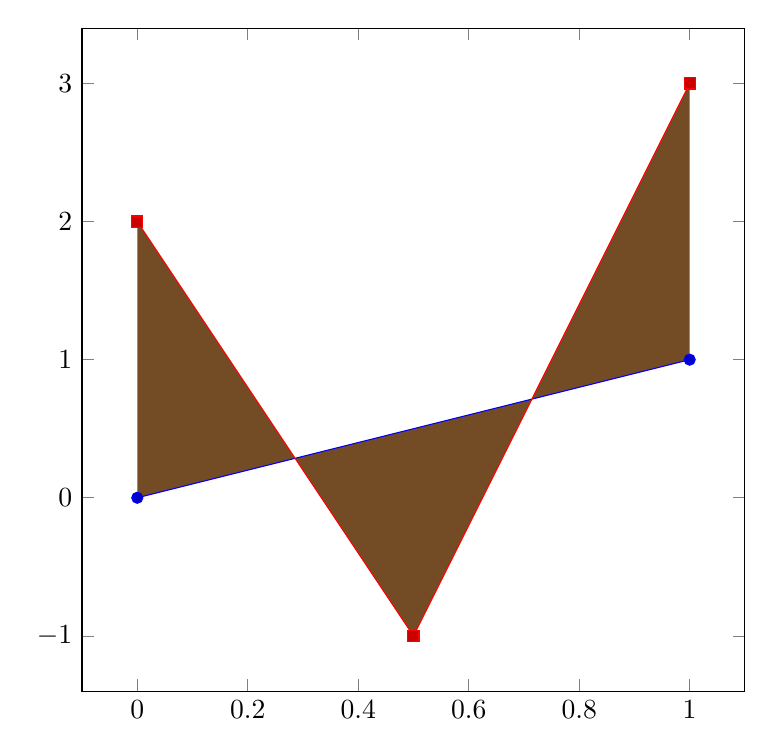
\begin{tikzpicture}\begin{axis}

\addplot+ [name path=A,domain=0:1,samples=2] {x};
\addplot+ [name path=B] table {
x y
0 2
0.5 -1
1 3
};
\addplot fill between [of=A and B];

\end{axis}\end{tikzpicture}\end{document}
